% !TEX root = main.tex
\documentclass [11pt,twoside]{article}
\usepackage[utf8]{inputenc}
\usepackage[T1]{fontenc}

%Page margins, header and footer positions
\usepackage{geometry}
 \geometry{
 a4paper,
 total={210mm,297mm},
 left=25mm,
 right=25mm,
 top=30mm,
 bottom=25mm,
 headsep=7mm}

\interfootnotelinepenalty=10000

%To display filling dots in the TOC for all entries
\usepackage[titles]{tocloft}
\renewcommand{\cftsecleader}{\cftdotfill{\cftdotsep}}

%Define new header and footer style
\usepackage{fancyhdr}

\pagestyle{fancy}
\fancyhf{}
\lhead{\color{Gray}{\small{BBP project by Angelo Cantoli, Simone Edmondo Bedini}}}
\lfoot{\textcolor{Gray}{\small{Copyright © 2025 - Angelo Cantoli, Simone Edmondo Bedini - All rights reserved}}}
\rfoot{\textcolor{Gray}{\thepage}}
\renewcommand{\headrulewidth}{0pt}

%PACKAGES
\usepackage{wasysym}
\usepackage{pifont}
\usepackage{minted}
\usepackage{subcaption}

\newcommand{\supported}{\ding{52}\xspace}
\newcommand{\unsupported}{\ding{55}\xspace}
\newcommand{\partsupported}{\textcolor{black!40}{\ding{52}}\xspace}
\newcommand{\lowsupported}{\textcolor{black!20}{\ding{52}}\xspace}
\newcommand{\unknowsupported}{\textbf{?}\xspace}

%Font: Times
\usepackage{times}
%Change monospaced font
\renewcommand{\ttdefault}{lmtt}

%tables
\usepackage{tabu}
\usepackage{tabularx}
\usepackage{ltablex}
\usepackage{longtable}
\usepackage{float} % To allow the use of H modifier in long tables

%landscape mode
\usepackage{pdflscape}
\usepackage{rotating}
\usepackage{caption}

%make landscape mode be sensitive to even and odd pages
%start
\def\myrotate{\ifodd\c@page\else-\fi 90}
\makeatletter
\global\let\orig@begin@landscape=\landscape%
\global\let\orig@end@landscape=\endlandscape%
\gdef\@true{1}
\gdef\@false{0}
\gdef\landscape{%
    \global\let\within@landscape=\@true%
    \orig@begin@landscape%
}%
\gdef\endlandscape{%
    \orig@end@landscape%
    \global\let\within@landscape=\@false%
}%
\@ifpackageloaded{pdflscape}{%
    \gdef\pdf@landscape@rotate{\PLS@Rotate}%
}{
    \gdef\pdf@landscape@rotate#1{}%
}
\let\latex@outputpage\@outputpage
\def\@outputpage{
    \ifx\within@landscape\@true%
        \if@twoside%
            \ifodd\c@page%
                \gdef\LS@rot{\setbox\@outputbox\vbox{%
                    \pdf@landscape@rotate{-90}%
                    \hbox{\rotatebox{90}{\hbox{\rotatebox{180}{\box\@outputbox}}}}}%
                }%
            \else%
                \gdef\LS@rot{\setbox\@outputbox\vbox{%
                    \pdf@landscape@rotate{+90}%
                    \hbox{\rotatebox{90}{\hbox{\rotatebox{0}{\box\@outputbox}}}}}%
                }%
            \fi%
        \else%
            \gdef\LS@rot{\setbox\@outputbox\vbox{%
                \pdf@landscape@rotate{+90}%
                \hbox{\rotatebox{90}{\hbox{\rotatebox{0}{\box\@outputbox}}}}}%
            }%
        \fi%
    \fi%
    \latex@outputpage%
}
\makeatother
%end

%graphics
\usepackage{graphicx}
\usepackage[dvipsnames, table]{xcolor}
%If you upload images from PC, you need to insert code for the path here (different for Windows and Unix OS)

%References
%\usepackage{xpatch}
%\usepackage[backend=biber, style=numeric, citestyle=numeric, sorting=none]{biblatex}
%\addbibresource{main.bib}

%Other
\usepackage{ifthen}
\usepackage{xspace}
\usepackage{enumitem}
\usepackage{amssymb}
\usepackage[pdftex, colorlinks, linkcolor=black, citecolor=black, urlcolor=blue]{hyperref}
\newcommand{\comment}[1]{{\color{Red}$\blacktriangleright$ Comment: #1 $\blacktriangleleft$}}


% Some utilities\ldots
\usepackage{soul}
\usepackage{tikz}

\usetikzlibrary{calc}
\usetikzlibrary{decorations.pathmorphing}


\makeatletter

\newcommand{\defhighlighter}[3][]{%
  \tikzset{every highlighter/.style={color=#2, fill opacity=#3, #1}}%
}

\defhighlighter{yellow}{.5}

\newcommand{\highlight@DoHighlight}{
  \fill [ decoration = {random steps, amplitude=1pt, segment length=15pt}
        , outer sep = -15pt, inner sep = 0pt, decorate
        , every highlighter, this highlighter ]
        ($(begin highlight)+(0,8pt)$) rectangle ($(end highlight)+(0,-3pt)$) ;
}

\newcommand{\highlight@BeginHighlight}{
  \coordinate (begin highlight) at (0,0);
}

\newcommand{\highlight@EndHighlight}{
  \coordinate (end highlight) at (0,0);
}

\newdimen\highlight@previous
\newdimen\highlight@current

\DeclareRobustCommand*\highlight[1][]{%
  \tikzset{this highlighter/.style={#1}}%
  \SOUL@setup
  %
  \def\SOUL@preamble{%
    \begin{tikzpicture}[overlay, remember picture]
      \highlight@BeginHighlight
      \highlight@EndHighlight
    \end{tikzpicture}%
  }%
  %
  \def\SOUL@postamble{%
    \begin{tikzpicture}[overlay, remember picture]
      \highlight@EndHighlight
      \highlight@DoHighlight
    \end{tikzpicture}%
  }%
  %
  \def\SOUL@everyhyphen{%
    \discretionary{%
      \SOUL@setkern\SOUL@hyphkern
      \SOUL@sethyphenchar
      \tikz[overlay, remember picture] \highlight@EndHighlight;%
    }{%
    }{%
      \SOUL@setkern\SOUL@charkern
    }%
  }%
  %
  \def\SOUL@everyexhyphen##1{%
    \SOUL@setkern\SOUL@hyphkern
    \hbox{##1}%
    \discretionary{%
      \tikz[overlay, remember picture] \highlight@EndHighlight;%
    }{%
    }{%
      \SOUL@setkern\SOUL@charkern
    }%
  }%
  %
  \def\SOUL@everysyllable{%
    \begin{tikzpicture}[overlay, remember picture]
      \path let \p0 = (begin highlight), \p1 = (0,0) in \pgfextra
        \global\highlight@previous=\y0
        \global\highlight@current =\y1
      \endpgfextra (0,0);
      \ifdim\highlight@current < \highlight@previous
        \highlight@DoHighlight
        \highlight@BeginHighlight
      \fi
    \end{tikzpicture}%
    \the\SOUL@syllable
    \tikz[overlay, remember picture] \highlight@EndHighlight;%
  }%
  \SOUL@
}

\makeatother

% Common abbrev. are set as commands to ensure proper spacing after the dot
\RequirePackage{xspace}
\newcommand{\ie}{i.e.\@\xspace}
\newcommand{\aka}{a.k.a.\@\xspace}
\newcommand{\Ie}{I.e.\@\xspace}
\newcommand{\cf}{cf.\@\xspace}
\newcommand{\Cf}{Cf.\@\xspace}
\newcommand{\eg}{e.g.\@\xspace}
\newcommand{\Eg}{E.g.\@\xspace}
\newcommand{\etal}{et al.\@\xspace}
\newcommand{\etc}{etc.\@\xspace}
\newcommand{\wrt}{w.r.t.\@\xspace}
\newcommand{\Wrt}{W.r.t.\@\xspace}



\date{}
\raggedbottom
\begin{document}

%TITLE PAGE

\begin{titlepage}


%LOGO

{\begin{table}[t!]
\centering
\begin{tabu} to \textwidth { X[1.3,r,p] X[1.7,l,p] }
\textcolor{Blue}
{\begin{flushleft}\textbf{Angelo Cantoli - Simone Edmondo Bedini}\end{flushleft}} & \begin{flushright}
\includegraphics[scale=0.45]{Images/PolimiLogo}\end{flushright}
\end{tabu}
\end{table}}~\\ [7cm]

%TITLE 

\begin{flushleft}

%Replace the text string with your title
{\textcolor{Blue}{\textbf{\Huge{Requirement Analysis and Specification
        Document}}}} \\ [1cm]

\end{flushleft}

\end{titlepage}

%Define deliverable specific info
%Replace cell contents where needed
\begin{table}[h!]
\begin{tabu} to \textwidth { X[0.3,r,p] X[0.7,l,p] }
\hline

\textbf{Deliverable:} & RASD\\
\textbf{Title:} & Requirement Analysis and Verification Document \\
\textbf{Authors:} & Angelo Cantoli, Simone Edmondo Bedini \\
\textbf{Version:} & 1.0 \\ 
\textbf{Date:} & 28/10/2025 \\
\textbf{Download page:} & https://github.com/angelo-cantoli/CantoliBedini \\
\textbf{Copyright:} & Copyright © 2025 - Angelo Cantoli, Simone Edmondo Bedini - All rights reserved \\
\hline
\end{tabu}
\end{table}




\setcounter{page}{2}


%------------------------------------------------------------------------------------------------------------------------------------------------
\newpage
\addcontentsline{toc}{section}{Table of Contents}
\tableofcontents
\newpage
\addcontentsline{toc}{section}{List of Figures}
\listoffigures
\addcontentsline{toc}{section}{List of Tables}
\listoftables

%------------------------------------------------------------------------------------------------------------------------------------------------
\clearpage
{\color{Blue}{\section{Introduction}}}\label{sect:introduction}
\subsection{Purpose}
BBP is a software designed to simplify the life of everyone who goes on bike trips and wants to enjoy them without worrying about finding the best routes.\\
It is intended as a community for cyclists, in which every person can share information about their personal routes, so that everyone may take advantage of the information and experience of other bikers.
The application is intended for smartphone, where it can make use of GPS and sensor data to seamlessly reconstruct the path a cyclist has taken.

\subsubsection{Goals}
\begin{itemize}
    \item G1: Users can record their bike trips through an automated process
    \item G2: Users can manually insert and record data about their bike trips
    \item G3: Users can view statistics and status of recorded bike trips
    \item G4: Users can access, if available, metereological data about the bike trip
    \item G5: Users can view potential hazards identified on the bike path
    \item G6: Users can publish recorded bike trips
    \item G7: Users can access all published bike trips
    \item G8: Users can view, on a map, all published bike paths between two points, ordered based on their score
\end{itemize}

\subsection{Scope}

\subsubsection{World Phenomena}
\begin{itemize}
    \item WP1: User goes on a bike trip
    \item WP2: User wants to register his bike trips
    \item WP3: User encounters obstacles
    \item WP4: User wants to find the best bike paths
    \item WP5: User wants to access information about bike paths
    \item WP6: Meteorological conditions change along the bike path
    \item WP7: User wants to share information about their bike paths
\end{itemize}

\subsubsection{Shared Phenomena}
\begin{itemize}
    \item SP1: User creates an account
    \item SP2: User logs in the account
    \item SP3: User records a bike trip
    \item SP4: Application stores inserted bike trip
    \item SP5: Application calculates and provides statistics about bike trips
    \item SP6: App retrieves meteorological informations along the path from an external service
    \item SP7: App adds meteorological informations to bike path data
    \item SP8: User insert status and name of the streets in the bike path
    \item SP9: User insert presence of obstacles along the path
    \item SP10: User let BBP acquire data from his mobile phone automatically
    \item SP11: BBP guess if the user is biking given their speed
    \item SP12: BBP collects GPS information from users phone to reconstruct the followed path
    \item SP13: BBP acquires data from users phone sensors to identify potential problems on the path
    \item SP14: User confirms information acquired automatically from BBP
    \item SP15: User corrects information acquired automatically from BBP
    \item SP16: User publishes collected information on BBP
    \item SP17: Any user asks BBP to visualize bike path on a map, specifying origin and destination
    \item SP18: BBP provides all shared information about selected bike paths to any user
    \item SP19: BBP computes score of a path based on status and effectiveness on reaching the destination  
    \item SP20: BBP visualizes all paths between the two point inserted by user, ordered based on the computed score
\end{itemize}

\subsection{Definitions, Acronyms, Abbreviations}
\subsection{Revision History}
\subsection{Reference Documents}
\subsection{Document Structure}

%------------------------------------------------------------------------------------------------------------------------------------------------
\clearpage
{\color{Blue}{\section{Overall Description}}}\label{sect:overview}
\subsection{Product Perspective}

\subsubsection{Class Diagrams}

\subsubsection{State Diagrams}

\subsubsection{Scenarios}

\textbf{User Creates an Account}\\
J. Doe is a frequent cyclist, and desires an application that gives them the opportunity to log their cycling 
activity, and find information about the best bike routes in his city. They find that BBP perfectly 
suits their needs, and proceed to install the application. The application at first only shows the 
path viewing functionality: J. Doe wants to also record their trips, so they proceed to the ‘sign up’ 
section. The system then asks them to set a username, email and password, which J. Doe inserts, along 
with some optional personal information that they choose not to include. Inserting the username ‘JD’, 
the system responds that this username has already been taken, and prompts to insert a new username. 
Upon insertion of a different username, which was not taken by any other user, the system notifies 
that an email was sent to the specified address with a code, which is required to complete the 
registration. Upon inserting the code, the system creates the new account, and J. Doe can begin 
using the complete application. \\
\newline
\textbf{Registered User Automatically Records a Trip}\\
J. Doe is about to go biking in their city. Before going out to get their bike, they decide that they 
want to record this trip using BBP, so they open the app, where they are logged in to their account, 
and initiate an automated recording of a new trip. The system starts acquiring GPS and sensor data 
from the smartphone, and waits until J. Doe starts biking: at that point, the speed detected by the 
system is high enough to start tracking the device in order to reconstruct the path. While biking, 
J. Doe encounters a pothole: their bike lurches to one side, and the system perceives from the mobile 
device’s sensors that an abnormal movement has occurred, therefore it notes that an obstacle was 
encountered in that location. At the end of their trip, J. Doe gets off their bike and stops the 
recording, at which BBP notifies that the trip was successfully saved to their trip record. \\
\newline
\textbf{Registered User Manually Records a Trip}\\
J.Doe has finished cycling along a new route they found in their city, and they want to save the path 
in BBP while it is still fresh in their memory, since they didn’t activate the automated recording 
before starting to bike. They go to the ‘manual trip insertion’ section of the application, which 
requests the insertion of a starting and ending location and time, and the names and status of all 
roads on the route, in the order in which they were traversed. Additionally the system gives the 
option to mark any obstacles encountered along the route: J. Doe remembers seeing some potholes on 
some of the roads, so they mark them. Once all the information has been inserted, they press ‘save trip’, 
at which point the system reconstructs the path from the provided data and saves the trip to J. Doe’s 
record. \\
\newline
\textbf{User Looks at Possible Bike Paths}\\
J. Doe wants to bike to a new attraction that has recently opened in their city. However, he has never 
been to that neighbourhood, so they want to see if they can find any paths that can quickly and easily 
take them there. They open the BBP and go to the ‘path viewing’ section: after inserting their current 
location as an origin, and the attraction’s location as a destination, the system searches for any published 
paths which are suitable for this route. It finds a couple of paths, and calculates a score for each 
one before displaying them on a map: the one with the highest score is highlighted. J. Doe selects the 
highlighted path and checks what additional information is provided: BBP shows that the path isn’t the 
most direct way to reach the destination, but it is relatively flat and devoid of obstacles. J. Doe then 
selects the next highest scoring path: this path is more direct, but has more obstacles and roads in 
worse conditions, thus scoring lower. J. Doe considers that they want to reach the destination as quickly 
as possible, and thinks that their mountain bike is sturdy enough to not care too much about the worse 
road conditions, therefore they press the ‘export path’ button and choose to export the path to Google 
Maps, so they may begin navigation.

\subsection{Product Functions}

\textbf{Sign up \& Login} \\
Users can access the app in two ways: 
\begin{itemize}
    \item Unregistered access: accessing the app without registering an account gives a user access to the 
    path visualization interface. By inserting a start and end location, the application will show on a map 
    all the paths between the two points, sorted based on their score (as described in detail in the 'Path 
    Visualization' product function).
    \item Registered access: the app also gives users the option to register a personal account. It will ask 
    the user to insert a username, e-mail and a password, along with some optional personal data (name, date 
    of birth, profile picture). If the username or email is already taken by another user, the system will 
    notify that a different username must be chosen. A verification email will be sent to the provided address 
    with an OTP, which will be requested by the system before the registration can be submitted. Once the 
    registration is complete, the user can login to their account, which gives them the ability to record, and 
    eventually publish, their bike trips, in addition to the features of the unregistered access. The user can 
    log out from their account at any time. \\
\end{itemize}
\textbf{Recording of Trips} \\
The main functionality of BBP is to allow registered users to record and save their bike trips.
There are two ways to record a trip in BBP:
\begin{itemize}
    \item Manual recording: if the user wants to record their trip manually, they must insert all relevant 
    information into the BBP application: the start and end locations of their trip, the names of the streets 
    present in the path (in the order in which they were traversed), their status (selected from predefined 
    status values: optimal, medium, sufficient, requires maintenance), and the start and end times of the trip. 
    Users can also manually mark the locations of obstacles encountered along the path. The system will 
    reconstruct the path based on the streets provided and their order.
    \item Automatic recording: if the user wants to record their trip automatically, they must begin the 
    automated recording before the start of their trip, and allow BBP to acquire data from their mobile device. 
    BBP will then start tracking the GPS position of the user's mobile device to determine what path they are 
    taking; the tracking will begin once the speed of the mobile device is estimated to be elevated enough to 
    assume that they have started biking (e.g. 15 km/h), and will not end until the users manually halts the 
    recording. BBP will simultaneously access some of the mobile device's sensors, such as the gyroscope or 
    the accelerometer, so that if a notable movement is registered (due to the presence of some obstacle on 
    the road, such as a pothole) an obstacle marker is added to that point in the path. The system will also 
    determine the status of the road based on the number of obstacles and sensor data patterns. Once the trip 
    has ended the user must stop the recording, at which point BBP will save the trip.
\end{itemize}
The recorded trips are saved in a database accessible only to the user; trips can be published at any time so 
that other users may visualize them, however if the trip data was recorded automatically BBP will first ask 
the user to verify that the collected information is accurate, and if it is not to manually correct it by 
removing incorrect obstacle markers and adjusting the status of the roads, before publishing the trip. \\
\newline
\noindent
\textbf{Trip Statistics Generation} \\
Once a user has recorded a trip, the system will automatically generate some statistics about the trip. The 
statistics include:
\begin{itemize}
    \item total distance covered
    \item average speed
    \item time taken to complete the trip
    \item total elevation difference between start and end points
    \item effective elevation traversed
    \item average slope of the path 
\end{itemize}
These statistics are calculated based on the recorded path data and the inserted start/end times. The system 
will also query an external service to obtain meteorological data relative to the path at that time: if it is 
available, it will be added to the path statistics. The computed statistics are stored with the corresponding 
path in the database; the users have the option to access them when visualizing a path.
Additionally, the system will compute aggregate statistics across all the trips the user has recorded (e.g. 
average time taken to complete trips, average elevation difference of trips, etc.) \\
\newline
\textbf{Trip History Management} \\
Users have the option to view all their past recorded trips. The trips are presented in a list format in 
chronological order, with the date of recording, the name and the start and end locations immediately visible. 
By selecting a specific trip, the user can view the computed statistics for that trip, and a map view of the 
path: there is an option to open the path in a third party navigation app (e.g. Google Maps), so that the user 
can navigate the same route again if they desire. 
The user has the option to edit or delete the trips at any time, and can also choose to publish the trip: if 
the data for the trip was automatically generated and the user has not yet reviewed it,  the system will 
prompt the user to verify and correct the information before publishing. If a trip that has already been 
published is deleted or modified, the system will propagate the action to the published trip (e.g. if a user 
deletes a published trip from their personal trip history, the trip will no longer be available to other users); 
the user also has the option to make a published trip private again at any time, immediately removing it from 
public availability. \\
\newline
\textbf{Path Visualization} \\
Users, both registered and unregistered, can visualize published bike trips on a map. The application will 
prompt the user to insert a start and end location: once inserted, the system will search for all paths that 
connect those two points. The system then computes a score for each of the paths: the score is based on the 
status of the roads in the path, the time it would take for the user to reach the destination by following 
the path (calculated by considering the total length of the path and the elevation difference), the amount of 
obstacles along the path and the difficulty of the path (calculated by considering the average slope of the 
path). The system then shows the user all the identified paths on a map: the path with the highest score will 
be highlighted, while the others will be shown with lower opacity, and the scores will all be visible. Only 
the 5 paths with the highest score will be immediately visible, to avoid cluttering; the user will have the 
option to make all possible paths visible. The user can select a path by clicking on it: the application will 
then give the user the option to view the statistics of the path, select the path as the main highlighted path 
(if it isn't already), and to open the path in a third party navigation app (e.g. Google Maps). The user will 
also have the option to view all paths in a list, sorted by score.

\subsection{User Characteristics}
\subsubsection*{Unregistered User}
An unregistered user can use BBP in a reading-only way, visualizing paths on the map and their score to receive suggestions on which bike trip to take. 
Furthermore at every moment he can decide to register to take advantage of all the features of BBP.

\subsubsection*{Registered User}
A registered user is the main character of the app, and is fundamental for its correct functioning, because the database of routes of BPP is based on insertion of registered users. 
In fact, a registered user can visualize paths on the map like an unregistered user and they can also insert routes, manually or automatically, and make them public to let all users see them.


\subsection{Assumptions, Dependencies and Constraints}
\subsubsection{Domain Assumptions}
\begin{itemize}
    \item D1: Each registered user has a valid email address
    \item D2: Users have a mobile device capable of running the BBP application
    \item D3: Users' mobile devices have GPS capabilities, with typical smartphone precision (5-10 meters)
    \item D4: GPS signals are generally available with sufficient precision while cycling
    \item D5: Registered users who use the automated recording functionality have accelerometer and gyroscope sensors in their mobile devices
    \item D6: Users' have internet access when using online features (e.g. path publication and visualization, weather data retrieval)
    \item D7: Users bike on roads intended for cycling (where bike tracks exist, or cars are rare and speed limits are compatible with biking)
    \item D8: Users who manually record trips bike on named roads which are marked on maps
    \item D9: A sufficient number of registered users are willing to publish their bike routes
    \item D10: Obstacles on bike paths cause a significant enough shift in movement to be detectable through the mobile device's sensors
    \item D11: Users can assess road surface conditions and categorize them in the predefined status values
    \item D12: Bike paths can be reconstructed reasonably accurately based on the names of the streets and the order in which they were traversed
\end{itemize}

\subsubsection{Dependencies}
\subsubsection*{Mapping and routing service}
The BBP system depends on an external mapping and routing service (e.g GoogleMaps, OpenStreetMap, etc.) for tracking and visualizing the bike paths.
\subsubsection*{Meteorological service}
The BBP system depends on an external, third-party meteorological service to acquire data relative to the weather conditions on the bike paths, which are then used to enrich the data about the path.


%------------------------------------------------------------------------------------------------------------------------------------------------
\clearpage
{\color{Blue}{\section{Specific Requirements}}}\label{sect:requirements}
\subsection{External Interface Requirements}

\subsection{Functional Requirements}

\subsubsection{Mapping on requirements}

\subsubsection{Use case diagrams}

\subsubsection{Use cases}

\subsubsection*{  UC1. Unregistered user signs up}

\begin{table}[H]
   \begin{tabularx}{\textwidth}{|p{3cm}|X|}
   \hline
   \textbf{Actor} & Unregistered user \\ \hline
   \textbf{Entry conditions} & User is on login page of BBP \\ \hline
   \textbf{Event flow} & 
   1. User clicks to register on BBP \newline 
   2. BBP asks user to insert his informations for the account \newline
   3. User inserts his informations \newline
   4. BBP validates the inserted personal informations \newline
   5. BBP sends the registration outcome 
   \\ \hline
   \textbf{Exit conditions} & An account is created \\ \hline
   \textbf{Exceptions} & Username already taken \newline Password not valid \newline Connection error while registering \\ \hline
   \end{tabularx}
\end{table}

\begin{figure}[H]
    \centering
    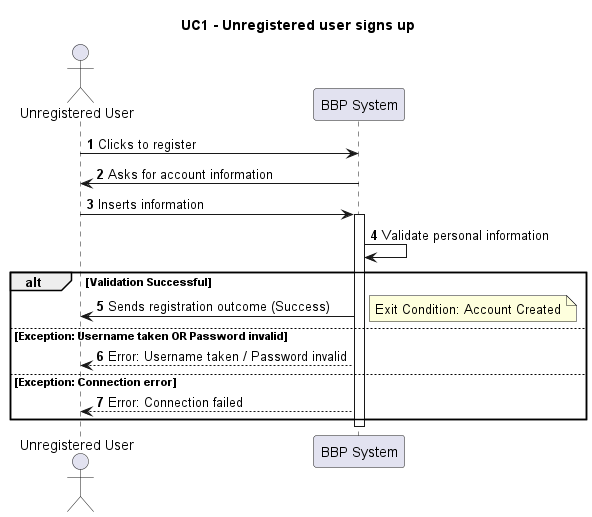
\includegraphics[width=0.9\textwidth]{./out/RASD/uml/UC1/UC1_SignUp.png}
    \caption{Use Case Diagram for UC1: Unregistered user signs up}
\end{figure}

\subsubsection*{  UC2. User logs in the account}

\begin{table}[H]
   \begin{tabularx}{\textwidth}{|p{3cm}|X|}
   \hline
   \textbf{Actor} & Registered user \\ \hline
   \textbf{Entry conditions} & Unregistered is on login page of BBP \\ \hline
   \textbf{Event flow} & 
   1. User clicks to login on BBP \newline
   2. BBP asks user to insert username and password of the account he wants to log in \newline
   3. User inserts his username \newline
   4. BBP validates the inserted username and password \newline
   5. BBP sends login outcome
   \\ \hline
   \textbf{Exit conditions} & User logs BBP system \\ \hline
   \textbf{Exceptions} & Inserted username not existent \newline Wrong inserted password for specified username \newline Connection error while logging in \\ \hline
   \end{tabularx}
\end{table}

\begin{figure}[H]
    \centering
    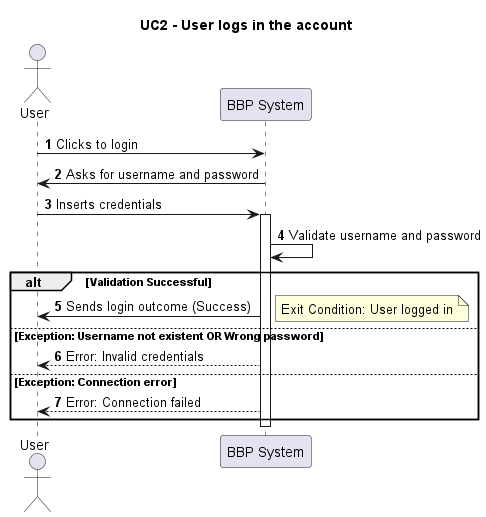
\includegraphics[width=0.9\textwidth]{./out/RASD/uml/UC2/UC2_Login.png}
    \caption{Use Case Diagram for UC2: User logs in the account}
\end{figure}

\subsubsection*{  UC3. User manually adds bike trip}

\begin{table}[H]
   \begin{tabularx}{\textwidth}{|p{3cm}|X|}
   \hline
   \textbf{Actor} & Registered user \\ \hline
   \textbf{Entry conditions} & User is registered and logged in \newline User is on "New trip" page \\ \hline
   \textbf{Event flow} &
   1. User clicks on "Insert a bike trip" button \newline
   2. BBP asks to insert a name for the trip \newline
   3. User inserts name of the trip \newline
   4. BBP validates inserted name \newline
   5. User inserts traveled roads \newline
   6. BBP calculate and returns the complete traveled route \newline
   7. User confirms calculated route \newline
   8. User inserted optional information, i.e obstacles \newline
   9. BBP calculates status based on inserted informations and shows to user \newline
   10. User clicks "Save trip" button \newline
   11. BBP saves trip, and informs user of outcome
   \\ \hline
   \textbf{Exit conditions} & Inserted trip is saved \\ \hline
   \textbf{Exceptions} & BBP can't calculate a route based on inserted roads \newline User already saved a route with the same name \\ \hline
   \end{tabularx}
\end{table}

\begin{figure}[H]
    \centering
    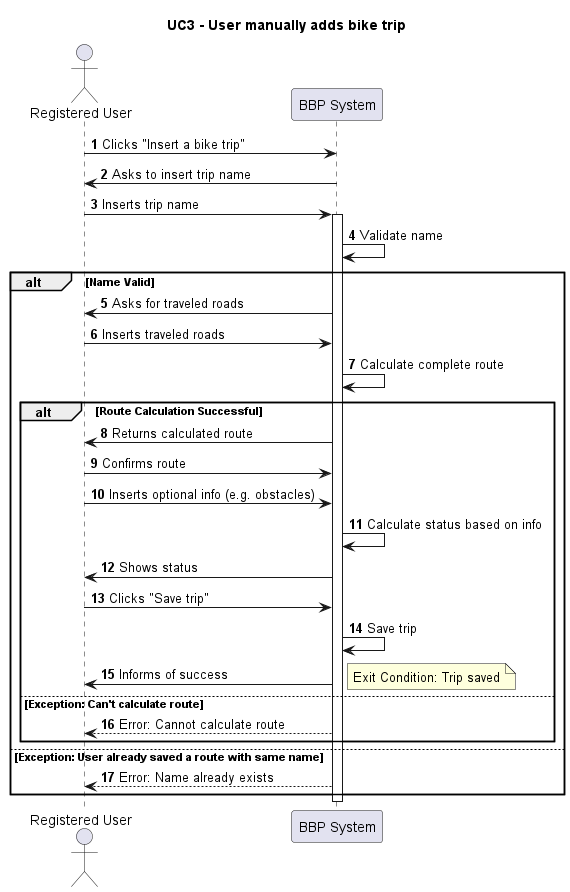
\includegraphics[width=0.9\textwidth]{./out/RASD/uml/UC3/UC3_ManualAdd.png}
    \caption{Use Case Diagram for UC3: User manually adds bike trip}
\end{figure}

\subsubsection*{  UC4. User automatically records bike trip}

\begin{table}[H]
   \begin{tabularx}{\textwidth}{|p{3cm}|X|}
   \hline
   \textbf{Actor} & Registered user \\ \hline
   \textbf{Entry conditions} & User is registered and logged in \newline User is on "New trip" page \\ \hline
   \textbf{Event flow} &
   1. User clicks to start automatic recording mode \newline
   2. BBP starts taking data from user's phone GPS \newline
   3. BBP recognize user is cycling, based on his velocity from sensors \newline
   4. BBP traces position and encountered obstacles with user's phone sensors and GPS \newline
   5. BBP recognize user stopped cycling \newline
   6. User finished automatic recording \newline
   7. BBP asks user to confirm or correct recorded data \newline
   8. User optionally corrects data and click confirm \newline
   9. BBP calculate status based on recorded and inserted data and shows to user \newline
   10. User insert a name for the trip and clicks "Save trip" button \newline
   11. BBP saves trip, and informs user of outcome
   \\ \hline
   \textbf{Exit conditions} & Recorded trip is saved \\ \hline
   \textbf{Exceptions} & GPS signal lost \newline Sensor permissions negated \newline User already saved a route with the same name \newline User discards recorded trip \\ \hline
   \end{tabularx}
\end{table}

\begin{figure}[H]
    \centering
    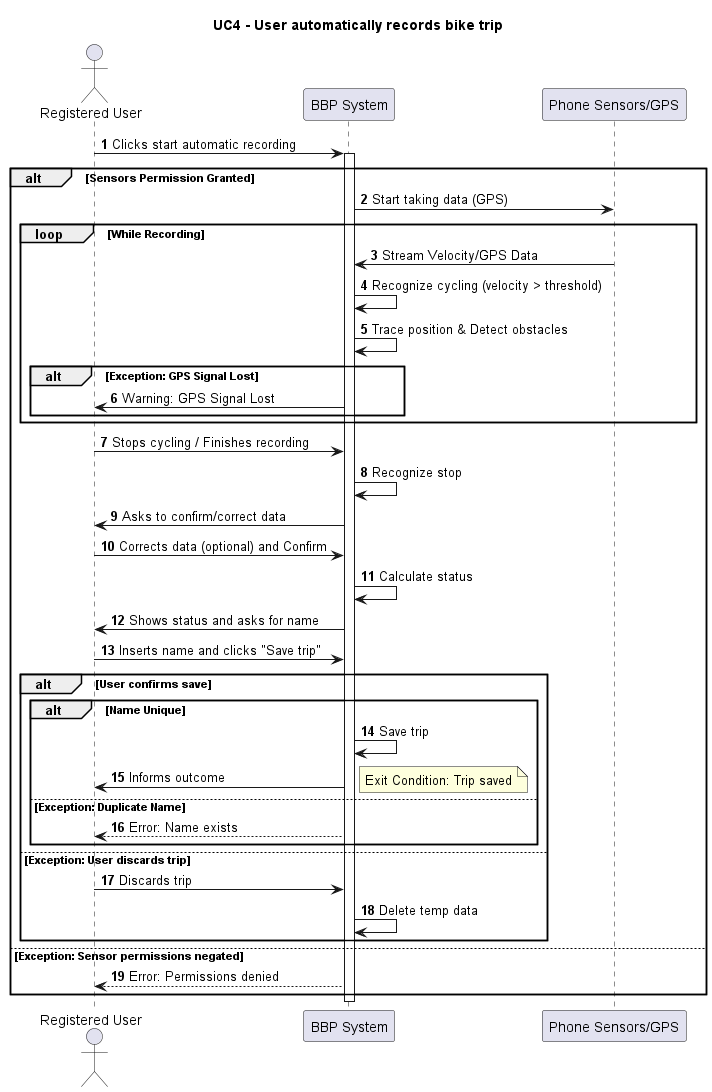
\includegraphics[width=0.9\textwidth]{./out/RASD/uml/UC4/UC4_AutoRecord.png}
    \caption{Use Case Diagram for UC4: User automatically records bike trip}
\end{figure}

\subsubsection*{  UC5. User views his bike trip history}

\begin{table}[H]
   \begin{tabular}{|p{3cm}|p{12cm}|}
   \hline
   \textbf{Actor} & Registered user \\ \hline
   \textbf{Entry conditions} & 
   User is registered and logged in \newline
   User is on "Your trips" page \\ \hline
   \textbf{Event flow} &
   1. User opens on "Bike trip history" section \newline
   2. BBP loads history of trips of user \newline
   3. User visualizes his trips
   \\ \hline
   \textbf{Exit conditions} & User closes "Bike trip history" section \\ \hline
   \textbf{Exceptions} & User does not have any saved trips \\ \hline
   \end{tabular}
\end{table}

\begin{figure}[H]
    \centering
    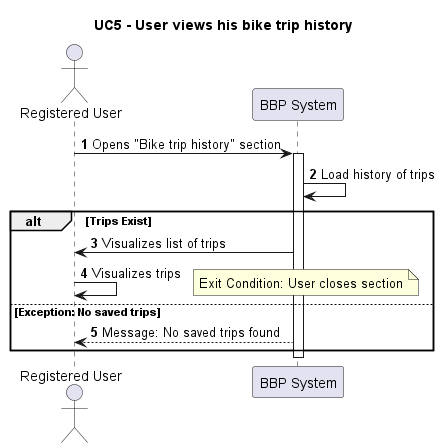
\includegraphics[width=0.9\textwidth]{./out/RASD/uml/UC5/UC5_ViewHistory.png}
    \caption{Use Case Diagram for UC5: User views his bike trip history}
\end{figure}

\subsubsection*{  UC6. User views his bike trip statistics}

\begin{table}[H]
   \begin{tabular}{|p{3cm}|p{12cm}|}
   \hline
   \textbf{Actor} & Registered user \\ \hline
   \textbf{Entry conditions} & 
   User is registered and logged in \newline
   User selected a specific trip from history \\ \hline
   \textbf{Event flow} &
   1. User clicks on "View statistics" button \newline
   2. BBP loads complessive statistics of traveled bike trips, and statistics for each trip \newline
   3. User clicks on a specific trip \newline
   4. BBP visualizes in-depth statistics for that trip
   \\ \hline
   \textbf{Exit conditions} & User closes "Trips Statistics" section \\ \hline
   \textbf{Exceptions} & User does not have any trip to calculate statistics on \\ \hline
   \end{tabular}
\end{table}

\begin{figure}[H]
    \centering
    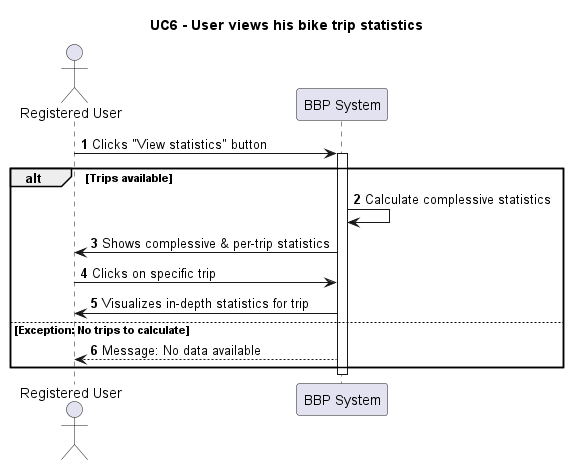
\includegraphics[width=0.9\textwidth]{./out/RASD/uml/UC6/UC6_ViewStats.png}
    \caption{Use Case Diagram for UC6: User views his bike trip statistics}
\end{figure}

\subsubsection*{  UC7. User publishes recorded trip}

\begin{table}[H]
   \begin{tabular}{|p{3cm}|p{12cm}|}
   \hline
   \textbf{Actor} & Registered user \\ \hline
   \textbf{Entry conditions} & 
   User is registered and logged in \newline
   User selected a specific trip from history \\ \hline
   \textbf{Event flow} &
   1. User click on "Publish trip" \newline
   2. BBP ask confirm to user if information are correct and if he is sure to make the trip public \newline
   3. User confirms the intention to publish \newline
   4. BBP publishes the trip, making it visible to all users
   \\ \hline
   \textbf{Exit conditions} & User's trip is published and visible by all users \\ \hline
   \textbf{Exceptions} & Connection error while publishing \\ \hline
   \end{tabular}
\end{table}

\begin{figure}[H]
    \centering
    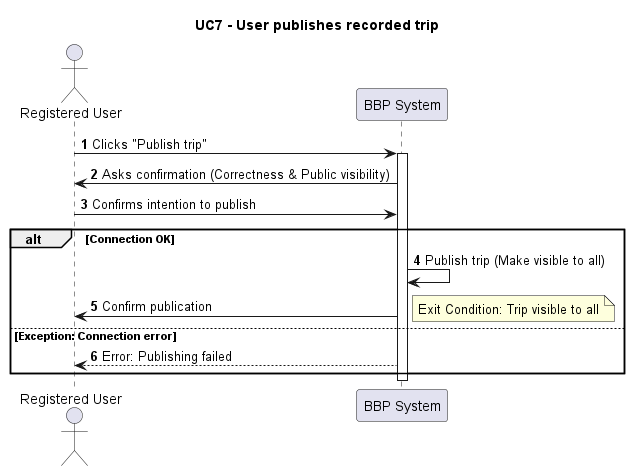
\includegraphics[width=0.9\textwidth]{./out/RASD/uml/UC7/UC7_PublishTrip.png}
    \caption{Use Case Diagram for UC7: User publishes recorded trip}
\end{figure}

\subsubsection*{  UC8. User modify one of his saved trips}

\begin{table}[H]
   \begin{tabular}{|p{3cm}|p{12cm}|}
   \hline
   \textbf{Actor} & Registered user \\ \hline
   \textbf{Entry conditions} & 
   User is registered and logged in \newline
   User selected a specific trip from history \\ \hline
   \textbf{Event flow} &
   1. User click on "Modify trip" \newline
   2. BBP allows users to modify saved data about trip \newline
   3. User modifies trip data \newline
   4. BBP validate changes of trip data \newline
   5. User confirm the changes of trip data \newline
   6. BBP modifies trip data on database and if the trip is public propagates changes for every user
   \\ \hline
   \textbf{Exit conditions} & Trip data is modified \\ \hline
   \textbf{Exceptions} & Inserted data is not valid \newline Connection error while propagating changes of public trip\\ \hline
   \end{tabular}
\end{table}

\begin{figure}[H]
    \centering
    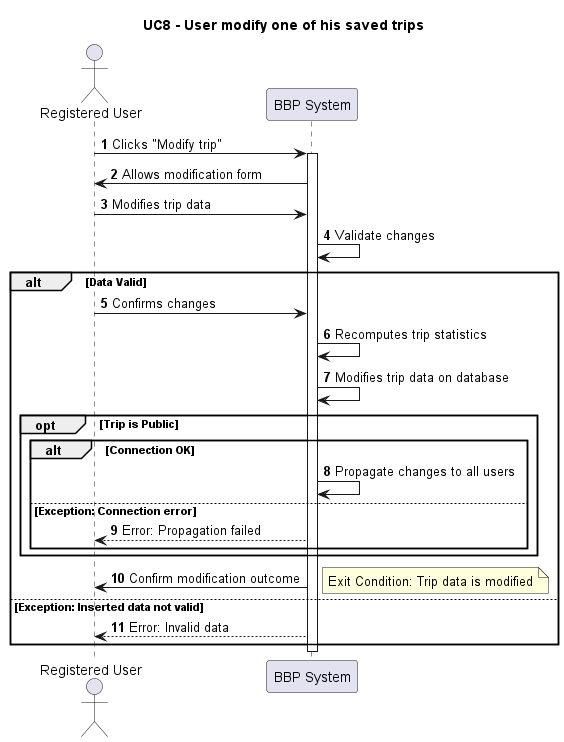
\includegraphics[width=0.9\textwidth]{./out/RASD/uml/UC8/UC8_ModifyTrip.png}
    \caption{Use Case Diagram for UC8: User modifies one of his saved trips}
\end{figure}

\subsubsection*{  UC9. User views possible bike routes on map}

\begin{table}[H]
   \begin{tabular}{|p{3cm}|p{12cm}|}
   \hline
   \textbf{Actor} & Registered user \newline Unregistered user \\ \hline
   \textbf{Entry conditions} & 
   User is on "Path search" section \\ \hline
   \textbf{Event flow} &
   1. BBP asks user to insert start and end point of route \newline
   2. User inserts start and end point \newline
   3. BBP visualizes every routes, with related score, between selected points
   \\ \hline
   \textbf{Exit conditions} & Paths are visualized \\ \hline
   \textbf{Exceptions} & Mapping service unavailable \newline Connection error while retrieving paths \newline No route found between the selected points \\ \hline
   \end{tabular}
\end{table}

\begin{figure}[H]
    \centering
    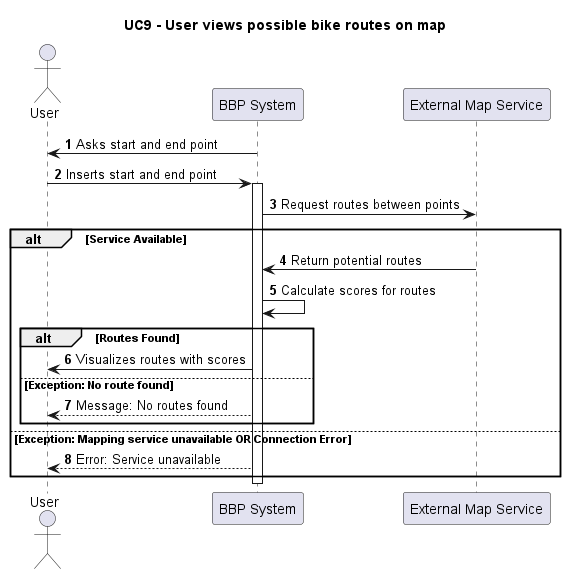
\includegraphics[width=0.9\textwidth]{./out/RASD/uml/UC9/UC9_ViewMapRoutes.png}
    \caption{Use Case Diagram for UC9: User views possible bike routes on map}
\end{figure}

\subsubsection*{  UC10. User views additional information about selected path on map}

\begin{table}[H]
   \begin{tabular}{|p{3cm}|p{12cm}|}
   \hline
   \textbf{Actor} & Registered user \newline Unregistered user \\ \hline
   \textbf{Entry conditions} & 
   User is on "Path search" section visualizing paths between 2 points \\ \hline
   \textbf{Event flow} &
   1. User clicks on a specific path on the map \newline
   2. BBP shows details about trip, i.e statistics, distance, obstacles etc..
   \\ \hline
   \textbf{Exit conditions} & Additionals informations of a trip are visualized \\ \hline
   \textbf{Exceptions} \\ \hline
   \end{tabular}
\end{table}

\begin{figure}[H]
    \centering
    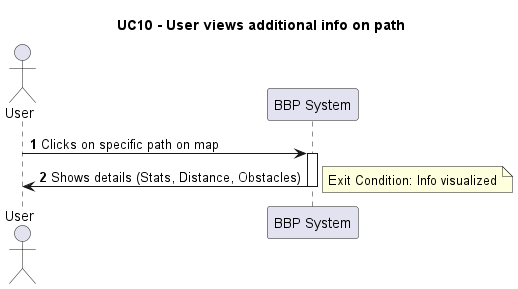
\includegraphics[width=0.9\textwidth]{./out/RASD/uml/UC10/UC10_ViewPathDetails.png}
    \caption{Use Case Diagram for UC10: User views additional information about selected path on map}
\end{figure}

\subsubsection*{  UC11. User start navigation on selected bike path}

\begin{table}[H]
   \begin{tabular}{|p{3cm}|p{12cm}|}
   \hline
   \textbf{Actor} & Registered user \newline Unregistered user \\ \hline
   \textbf{Entry conditions} & 
   User selected a path on the map \\ \hline
   \textbf{Event flow} &
   1. User click to open route on a third-party mapping service \newline
   2. BBP opens third-party mapping service, giving it coordinates of start and end point
   \\ \hline
   \textbf{Exit conditions} & Additionals informations of a trip are visualized \\ \hline
   \textbf{Exceptions} & hird-party mapping service not available\\ \hline
   \end{tabular}
\end{table}

\begin{figure}[H]
    \centering
    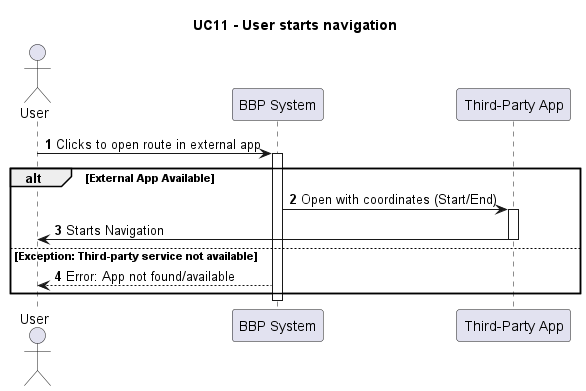
\includegraphics[width=0.9\textwidth]{./out/RASD/uml/UC11/UC11_StartNav.png}
    \caption{Use Case Diagram for UC11: User start navigation on selected bike path}
\end{figure}

\subsubsection*{  UC12. User modifies profile data}

\begin{table}[H]
   \begin{tabular}{|p{3cm}|p{12cm}|}
   \hline
   \textbf{Actor} & Registered user \\ \hline
   \textbf{Entry conditions} & 
   User is registered and logged in \newline
   User is on profile page of BPP \\ \hline
   \textbf{Event flow} &
   1. User clicks on modify profile data \newline
   2. User insert new personal data \newline
   3. BBP validates new personal data \newline
   4. User confirms changes on personal data \newline
   5. BBP update user personal data
   \\ \hline
   \textbf{Exit conditions} & User personal data are modified \\ \hline
   \textbf{Exceptions} & New username already taken \newline New password not valid \newline Connection error while modifying profile data \\ \hline
   \end{tabular}
\end{table}

\begin{figure}[H]
    \centering
    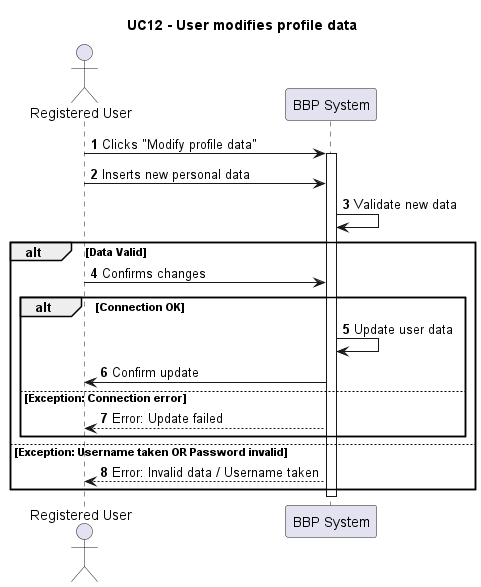
\includegraphics[width=0.9\textwidth]{./out/RASD/uml/UC12/UC12_ModifyProfile.png}
    \caption{Use Case Diagram for UC12: User modifies profile data}
\end{figure}

\subsubsection*{  UC13. User logs out the account}

\begin{table}[H]
   \begin{tabular}{|p{3cm}|p{12cm}|}
   \hline
   \textbf{Actor} & Registered user \\ \hline
   \textbf{Entry conditions} & 
   User is registered and logged in \\ \hline
   \textbf{Event flow} &
   1. User clicks on log out button \newline
   2. BBP terminate access of user on the account \newline
   3. BBP returns user to log in page
   \\ \hline
   \textbf{Exit conditions} & User is disconnected from the account \\ \hline
   \textbf{Exceptions} \\ \hline
   \end{tabular}
\end{table}

\begin{figure}[H]
    \centering
    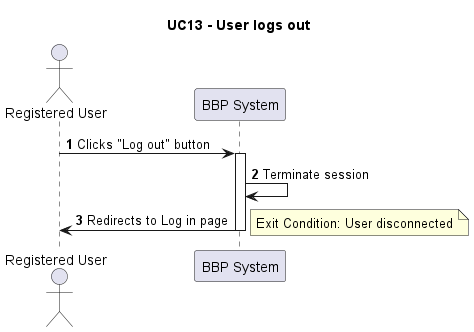
\includegraphics[width=0.9\textwidth]{./out/RASD/uml/UC13/UC13_Logout.png}
    \caption{Use Case Diagram for UC13: User logs out the account}
\end{figure}

%------------------------------------------------------------------------------------------------------------------------------------------------
\clearpage
{\color{Blue}{\section{Formal Analysis Using Alloy}}}\label{sect:alloy}
\subsection{Alloy Code}


    
\begin{minted}{Alloy}
open util/integer
open util/ordering[TimeStamp]

// SIGNATURES ----------------------------------------------------

sig User {}

sig RegisteredUser extends User {
    var records: disj set Trip,
    generates: disj AggregateStatistics,
    has: disj MobileDevice
}

sig Trip {
    mode: RecordingMode,
    var isPublished: Bool,
    var isVerified: Bool,
    generates: disj Statistics,
    traverses: disj Path,
    enrichedBy: disj lone MeteorologicalData,
    startTime: TimeStamp,
    endTime: TimeStamp
} {
    lt[startTime, endTime]
}

sig AggregateStatistics {
} {
    this in RegisteredUser.generates
}

sig Statistics {
} {
    this in Trip.generates
}

sig Path {
    composedBy: seq PathSegment
} {
    this in Trip.traverses and
    #composedBy > 0
}

sig PathSegment {
    contains: disj set Obstacle,
    starts: Location,
    ends: Location,
    status: RoadStatus
} {
    this in Path.composedBy.elems and
    starts != ends
}

sig Obstacle {
    positioned: Location
} {
    this in PathSegment.contains
}

sig MeteorologicalData {
} {
    this in Trip.enrichedBy
}

sig MobileDevice {
    contains: disj some Sensor
} {
    this in User.has
}

sig Sensor {
    type: SensorType
} {
    this in MobileDevice.contains
}

sig Location {
} {
    this in PathSegment.starts or
    this in PathSegment.ends or
    this in Obstacle.positioned
}

sig TimeStamp {
} {
    this in Trip.startTime or
    this in Trip.endTime
}

enum RecordingMode {MANUAL, AUTOMATED}

enum RoadStatus {OPTIMAL, MEDIUM, SUFFICIENT, REQUIRES_MAINTENANCE}

enum SensorType {GPS, GYRO, ACCELEROMETER}

enum Bool {TRUE, FALSE}


// FACTS ----------------------------------------------------

// A trip must be verified in order to be published
fact PublishedTripMustBeVerified {
    always(
        all t: Trip |
        (t.mode = AUTOMATED and t.isPublished = TRUE) implies 
        t.isVerified = TRUE
    )
}

// When trips are recorded, they are private
fact TripsStartNotPublished {
    all t: Trip |
        t.isPublished = FALSE and
        after always (
            t.isPublished = TRUE 
            implies
            once t.isPublished = FALSE
        )
}

// If an trip is recorded in automated mode, it is not verified 
// until the user corrects the data
fact TripsStartNotVerifiedIfAutomated {
    all t: Trip |
        t.mode = AUTOMATED implies (
            t.isVerified = FALSE and
            after always (
                t.isVerified = TRUE 
                implies
                once t.isVerified = FALSE
            )
        )
}

// Manually inserted trips do not need to be verified
fact ManualTripsVerified {
    always (
        all t: Trip |
            t.mode = MANUAL implies t.isVerified = TRUE
    )
}

// Path segments that compose a path must be connected
fact PathSegmentsAreConnected {
    all p: Path |
        all i: Int | 
            (i in p.composedBy.inds and i != p.composedBy.lastIdx) 
            implies  
            p.composedBy[i].ends = p.composedBy[add[i,1]].starts
}

// A user cannot have two trips that take place at the same time
fact NoConcurrentTrips {
    all u: RegisteredUser |
        all disj t1, t2: Trip |
            (t1 in u.records and t2 in u.records)
            implies
            (lte[t1.endTime, t2.startTime] or lte[t2.endTime, t1.startTime])
}

// All user's mobile devices have GPS functionalities
fact AllUsersHaveGPS {
    all u: RegisteredUser |
        one s: Sensor | s.type = GPS and s in u.has.contains
}


// Trips can be owned by only one user
fact TripsOwnedByOnlyOneUser {
    all t: Trip, u: RegisteredUser |
        t in u.records implies always(
            no u1: RegisteredUser | 
                u1 != u and t in u1.records
        )
}

// PREDICATES ----------------------------------------------------

pred recordTrip[u: RegisteredUser, t: Trip, m: RecordingMode] {
    no u2: RegisteredUser | t in u2.records
    t.mode = m

    u.records' = u.records + t
                     
    t.isPublished' = FALSE            
    
    all u1: RegisteredUser - u | u1.records' = u1.records
    
    all t1: Trip - t | {
        t1.isPublished' = t1.isPublished
        t1.isVerified' = t1.isVerified
    }
}

run recordTrip

pred verifyTrip[u: RegisteredUser, t: Trip] {
    t in u.records
    t.isVerified = FALSE

    t.isVerified' = TRUE

    -- Frame Conditions
    t.isPublished' = t.isPublished
    
    all u1: RegisteredUser | u1.records' = u1.records

    all t1: Trip - t | {
        t1.isPublished' = t1.isPublished
        t1.isVerified' = t1.isVerified
    }
}

run verifyTrip

pred publishTrip[u: RegisteredUser, t: Trip] {
    t in u.records
    t.isPublished = FALSE

    (t.mode = AUTOMATED) implies (t.isVerified = TRUE)

    t.isPublished' = TRUE

    -- Frame Conditions

    t.isVerified' = t.isVerified

    all u1: RegisteredUser | u1.records' = u1.records

    all t1: Trip - t | {
        t1.isPublished' = t1.isPublished
        t1.isVerified' = t1.isVerified
    }
}

run publishTrip

pred deleteTrip[u: RegisteredUser, t: Trip] {
    t in u.records

    u.records' = u.records - t

    -- Frame Conditions
    all u1: RegisteredUser - u | u1.records' = u1.records

    all t1: Trip - t | {
        t1.isPublished' = t1.isPublished
        t1.isVerified' = t1.isVerified
    }
}

run deleteTrip


pred showScenario {
    some disj u1, u2: RegisteredUser, disj t1, t2: Trip | {
        recordTrip[u1, t1, AUTOMATED]
        after verifyTrip[u1, t1]
        after after publishTrip[u1, t1]
        after after after recordTrip[u2, t2, MANUAL]
        after after after after deleteTrip[u2, t2]
    }
}

run showScenario for 5 but 3 Int, 6 TimeStamp
\end{minted}

%------------------------------------------------------------------------------------------------------------------------------------------------
\clearpage
{\color{Blue}{\section{Effort Spent}}}\label{sect:effort}
\begin{table}[h!]
\centering
\renewcommand{\arraystretch}{1.5} % Decommenta questa riga se vuoi le righe più spaziate
\begin{tabular}{c|l|c}
    \hline
    Member of group & \multicolumn{2}{c}{Effort spent} \\
    \hline
    Bedini Simone & Introduction & $9h$ \\
                                & Overall description & $10h$ \\
                                & Specific requirements & $11h$ \\
                                & Formal analysis & $15h$ \\
                                & Reasoning & $13h$ \\
    \hline
    Cantoli Angelo & Introduction & $9h$ \\
                                & Overall description & $11h$ \\
                                & Specific requirements & $24h$ \\
                                & Formal analysis & $2h$ \\
                                & Reasoning & $11h$ \\
    \hline
\end{tabular}
\end{table}

%------------------------------------------------------------------------------------------------------------------------------------------------
\clearpage
{\color{Blue}{\section{References}}}\label{sect:references}
\subsection{Reference Documents}

\begin{itemize}
   \item Assignment RDD AY 2025-2026.pdf
   \item Lecture slides and notes from the course Software Engineering 2 2025/2026
   \item Global Advisor-Cycling Across the World-2022 Report.pdf - \newline https://www.ipsos.com/sites/default/files/ct/news/documents/2022-05/Global%20Advisor-Cycling%20Across%20the%20World-2022%20Report.pdf
\end{itemize}

\subsection{Used Tools}
The following tools have been used to create this document:
\begin{itemize}
    \item \textbf{LaTeX}: for document preparation and typesetting.
    \item \textbf{PlantUML}: for creating UML diagrams included in the document.
    \item \textbf{GitHub}: for version control and collaboration on the document source files.
    \item \textbf{Alloy Analyzer}: for formal analysis and verification of system specifications.
    \item \textbf{VSCode}: as the main text editor for writing LaTeX code.
\end{itemize}


%------------------------------------------------------------------------------------------------------------------------------------------------
% \clearpage
% \addcontentsline{toc}{section}{References}
% \bibliographystyle{plain}
% \bibliography{main}
%------------------------------------------------------------------------------------------------------------------------------------------------




\end{document}